%!TEX root = ../Report.tex

In this chapter, we will explore the three key ideas requisite to this project, such that we can discuss how they are combined and the implications.

\section{What Is Co-Scheduling?}

It is known that in multiprogramming systems, with many programs running simultaneously, the choice of program to socket mapping significantly affects the performance of the system. (cite LIRA Section 2: Motivating Example) In the cite'd(?) case, just considering two programs running on the same socket, we can see from the graph in figure 2 (Cite) that certain programs perform differently with others, with some strange cases where the programs actually display better performance when running in contention with another.

So with this evidence, we can see that if we take into account these factors in our scheduler, we may obtain better overall performance. The outcome of the LIRA paper concludes that throughput gains of 3-7\% can be seen. Socket aware scheduling in this manner is called co-scheduling. Adding in the plastic programming idea could make this particularly powerful, because we know and control the specifics of the implementations, and not only can we control what program runs where, we can also adjust what implementation the program is using. As an example of how this would work in practice, see the following flow diagram:

\begin{center}
\vspace{0.5cm}
\includegraphics[width=1\textwidth]{co-scheduling_flow_diagram}
\end{center}

NOTE - CHANGE THIS GRAPH TO REFLECT FINAL IMPLEMENTATION

\section{What Is Plastic Programming?}

When programming an algorithm, there is often many choices about the specific implementation which can greatly affect performance, and the best choice depends on the circumstances of the problem. We tend to have more choices with parallel programs, but this is the case even for sequential programs. As an example, for a large input size, radix sort would perform best, whereas for a small input size, insertion sort would be better. So naturally, in the interests of performance, we can conceive of a better overall implementation by combining the two approaches, so while the task size is large we would use radix sort, and then once it is reduced we would use insertion sort. 

Such compositions are commonplace, such as the sorting example discussed in the PetaBricks paper (cite petabricks: Introduction, paragraph 2).

\begin{center}
	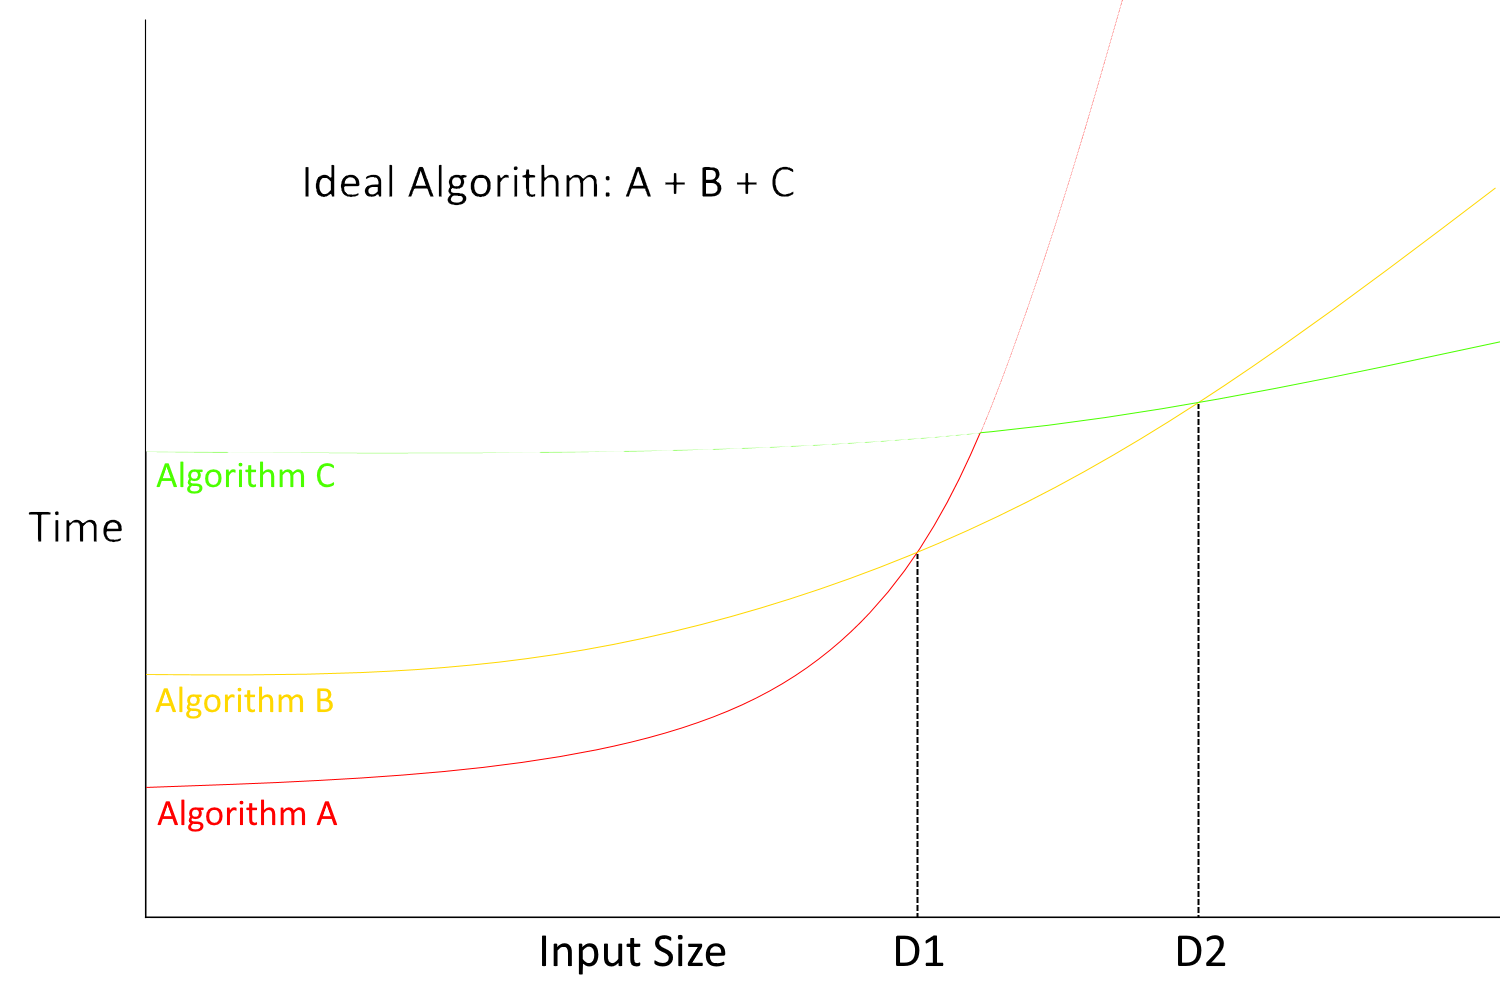
\includegraphics[width=0.8\textwidth]{plastic_graph}
\end{center}

\section{What Is Skeleton Programming?}

Skeleton programming is a high-level programming model. Skeletons allow us to abstract away all the complexity involved in parallel programming, plastic programming, and co-scheduling. The essence of skeleton programming is that the skeleton provides the core structure of an algorithm, the user provides some code (In our case, a function), which then produces a correct program for the task at hand. The skeleton handles the hard-work of providing and optimizing the code (In our case, dealing with parallelism, plasticity, and co-scheduling). The consequences of this are twofold:

\begin{itemize}
	\item Errors are reduced substantially, as parallel programming is not easy, even without plasticity and co-scheduling.
	\item We can assess the program's complexity, since we know the algorithmic details of the skeleton.
\end{itemize}

Typically, multiple skeletons are combined to produce a more complex program, for example, a common combination is Map and Reduce. The ability to combine skeletons makes them a powerful tool, allowing programmers to easily create clean complex programs.

\section{Summary}

The main new idea in this project is that of co-scheduling. It is an important factor in multiprogramming systems with performance implications. Plasticity is a technique to respond to this challenge, and take it further. This results in complex code, making it hard to ensure correctness. So we use skeletons to hide this complexity from the programmer. It also has the nice side effect of dividing the challenge into a pattern-by-pattern basis.

In this project we will produce such skeletons, and investigate the performance implications of these ideas, as it is not known whether they will have a significant effect.